\documentclass[a4paper, UKenglish, 11pt]{uiomaster}
\usepackage{lipsum}
\usepackage[subpreambles=true]{standalone}

\begin{document}

\chapter{Introduction to Neuroscience}
Sections ... and ... are based on the books Neuronal Dynamics by Gerstner, Kistler, Naud and Paninski \cite{gerstner2014neuronal} and Principles of computational modelling in neuroscience by Sterratt,Graham, Gillies, and Willshaw \cite{sterratt2011principles}.

% Cortex?
% Action potential ?

\section{The Neuron}

Neurons are the fundamental units of the central nervous system, forming intricate networks with numerous interconnections. Similar to other cells, neurons have a voltage difference across their cell membrane known as the membrane potential. This membrane potential is essential for signal transmission and processing, allowing neurons to communicate over long distances. At rest, the membrane potential of a neuron typically hovers around -65 mV, indicating that the interior of the cell is negatively charged compared to the external environment \cite{sterratt2011principles}.

A neuron consists of three distinct parts: the dendrites, the soma, also reffered to as the cell body, and the axon. Dendrites, with their branching structure, play an important role in collecting signals from other neurons. These signals are transmitted to the soma, which acts as the central processing unit, performing essential nonlinear processing. If the total input received by the soma reach a specific threshold, an action potential is generated. This signal generates an electrical current that travels along the axon, leading to the release of neurotransmitters. These neurotransmitters diffuse across the junction, or the synapse, between the sending and receiving neuron. If the receptors on the receiving neuron accept the neurotransmitters, a new electrical signal is generated. This transmission of signals between neurons at specialized junctions is called synaptic inputs.\cite{gerstner2014neuronal}

The neuron sending the synaptic input is referred to as the presynaptic cell, while the neuron receiving the synaptic input is called the postsynaptic cell. In vertebrates, a presynaptic neuron often connects to more than $10^4$ postsynaptic neurons. While many axonal branches terminate near the neuron itself, the axon can also extend over several centimeters to reach neurons in other regions of the brain \cite{gerstner2014neuronal}.

In figure \ref{fig:neuron} we have provided the basic arcitecture of the neuron.

\begin{figure}
    \centering
    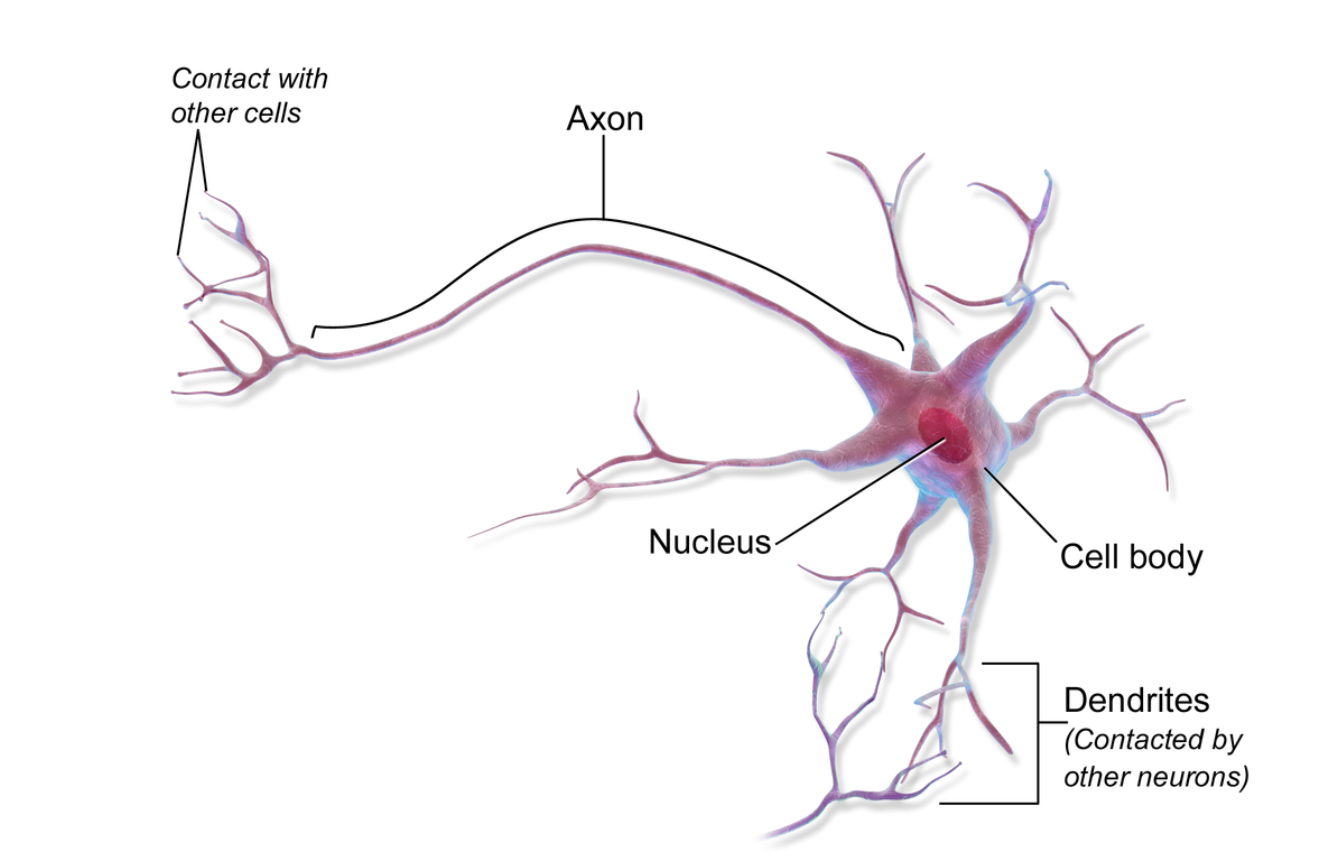
\includegraphics[width=\linewidth]{figures/neuron.png}
    \caption{An illustation of a single neuron with dendrites, soma (cell body) and axon. The figure is taken from ...}
    \label{fig:neuron}
\end{figure}

If the electrical signals that transmit towards the soma reach a certain treshold, usually around -55 mV, the neuron fires, and we say that an action potential is initiated. These action potentials or spikes, typically have an amplitude of about 100 mV and a duration of 1-2 ms \cite{gerstner2014neuronal}. As the form of isolated spikesof a given neuron more or less is the same through the propagation along the axon, the information of in these signals does not lay in the shape of the signal. Rather, we can from spike trains - chains of action potentials emitted by single neurons - collect information by looking at the number and timing of spikes. Figure \ref{fig:neuron} depicts multiple membrane potential recordings.

\begin{figure}
    \centering
    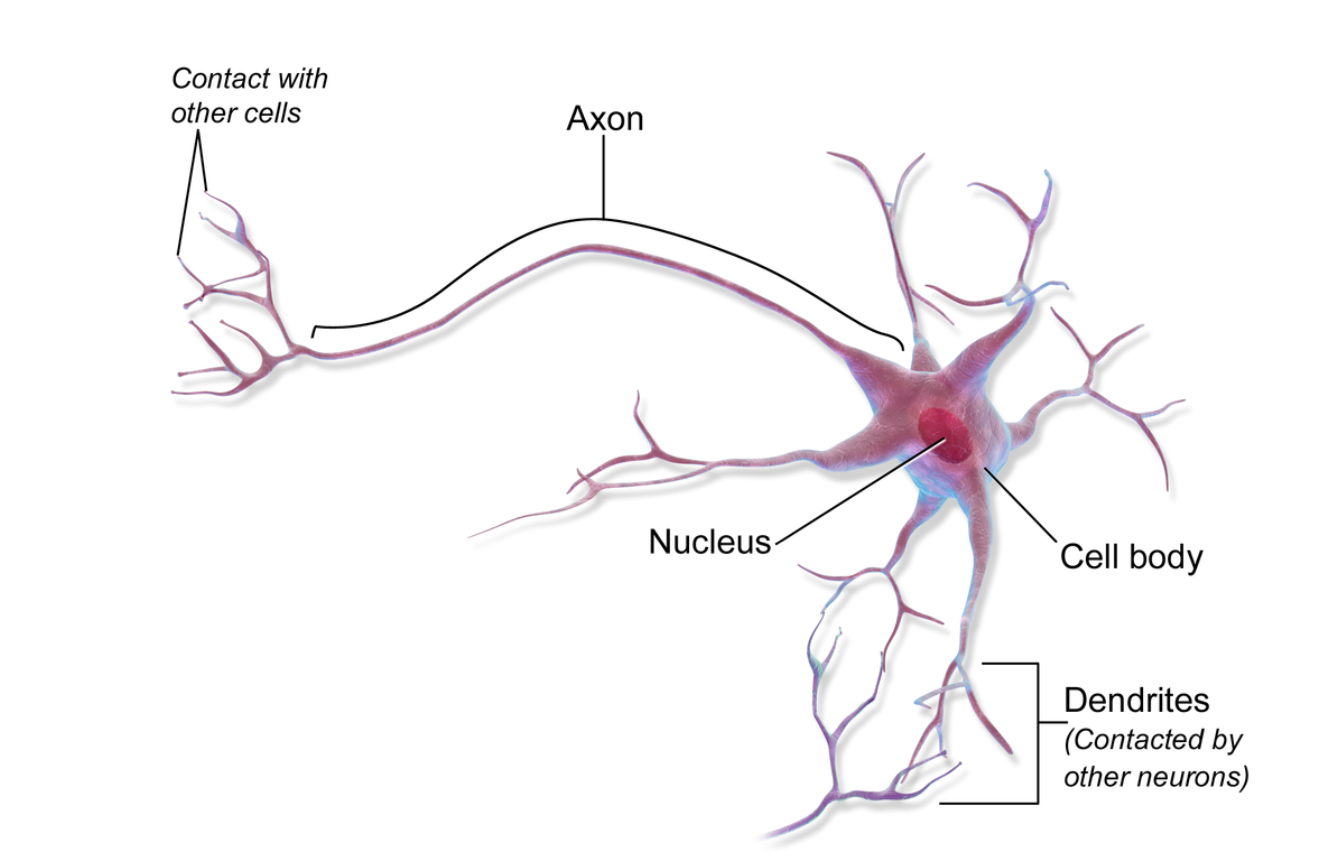
\includegraphics[width=\linewidth]{figures/neuron.png}
    \caption{An illustation of a single neuron with dendrites, soma (cell body) and axon. The figure is taken from ...}
    \label{fig:neuron}
\end{figure}


% Neurons are the fundamental units of the central nervous system, forming intricate networks with numerous interconnections. They possess a unique architecture that allows them to transmit and process signals. A neuron consists of three main components: dendrites, the soma (cell body), and the axon. Together, these parts enable the neuron to receive, integrate, and transmit electrical signals.
%
% Dendrites, with their branching structure, serve as the primary receivers of signals from other neurons. They collect incoming electrical impulses and transmit them towards the soma. The soma acts as the central processing unit of the neuron, where various computations take place. It integrates the incoming signals and, if the combined input reaches a specific threshold, initiates an action potential.
%
% An action potential, also known as a spike, is a brief electrical event that occurs when the neuron fires. It is characterized by a rapid change in membrane potential. Once initiated, the action potential generates an electrical current that travels along the axon, a long fiber-like extension of the neuron. The axon allows the electrical signal to propagate over long distances, facilitating communication between different parts of the nervous system.
%
% At the end of the axon, the electrical signal triggers the release of neurotransmitters into the synapse, the junction between the sending neuron (presynaptic cell) and the receiving neuron (postsynaptic cell). Neurotransmitters are chemical messengers that diffuse across the synapse and bind to receptors on the postsynaptic neuron. This binding generates a new electrical signal in the postsynaptic neuron, continuing the transmission of information.
%
% Figure \ref{fig:neuron} illustrates the basic architecture of a neuron, depicting the dendrites, soma, and axon.
%
% \begin{figure}
% \centering
% 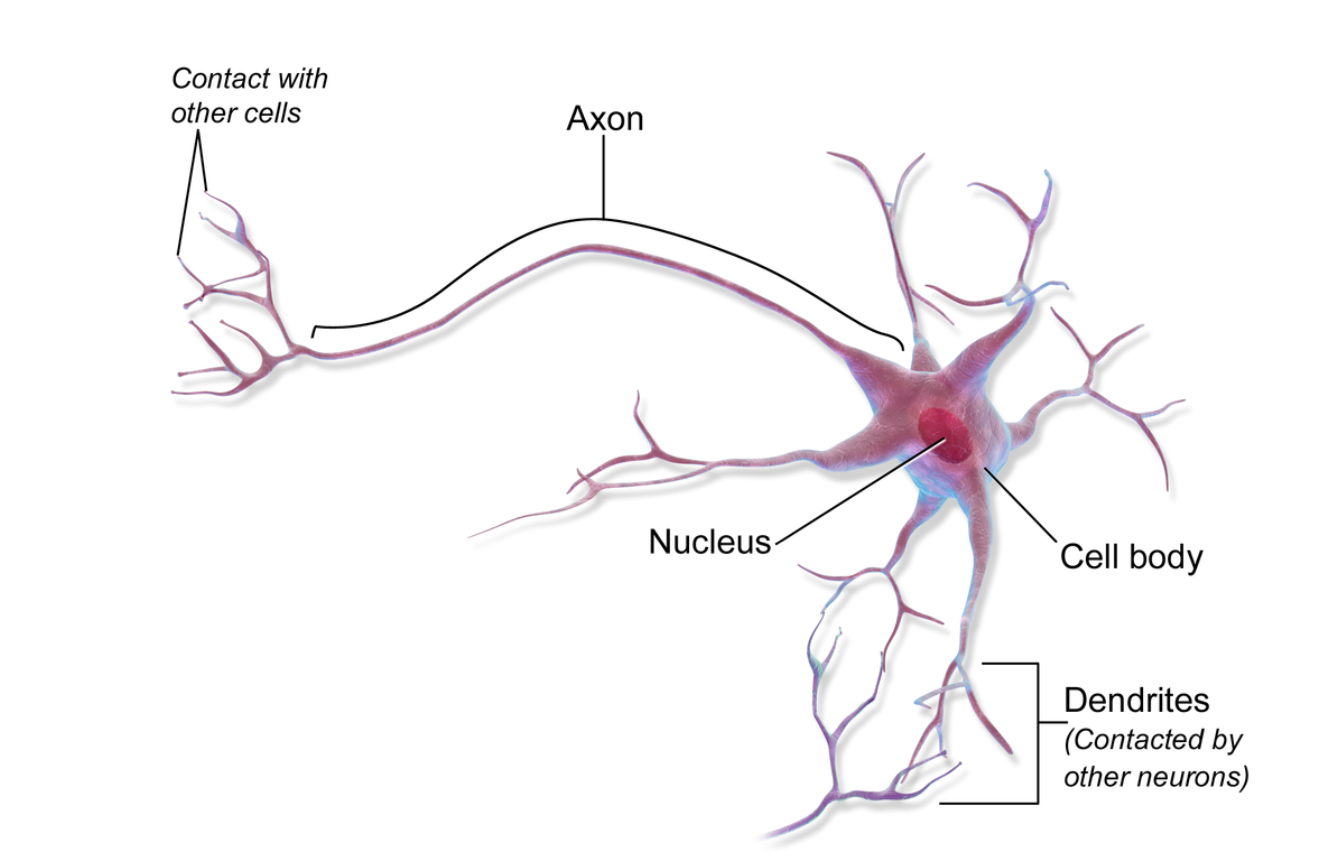
\includegraphics[width=\linewidth]{figures/neuron.png}
% \caption{An illustration of a single neuron with dendrites, soma (cell body), and axon.}
% \label{fig:neuron}
% \end{figure}
%
% It is important to note that the information in neuronal communication is not primarily encoded in the shape of individual spikes. Instead, meaningful information can be derived from analyzing patterns of spike trains, which are chains of action potentials emitted by single neurons. By examining the number and timing of spikes in these trains, researchers can gain insights into the underlying neuronal activity and information processing.



\section{Head Models and Multicompartmental Modeling }
% Something more about volume conducters

\section{Currents and Potentials in the Brain}
Ohm's law in volume conductors is a more genral statement than its usual form in electrical circuits. It is a linear relationship between vector current density $J$ and the electric field $E$. The law is then expessed as follows:

\begin{equation}
J = \sigma E,
\label{eq:ohms_law}
\end{equation}

where $\sigma$ is the conductivity of the .... (physical material). (Soruce: Electric Fields of the Brain: The Neurophysics of EEG).


































\section{Electroencephalograpy}
\section{EEG Forward modeling}
\section{The Inverse Problem}
\end{document}